%Configuracion del tipo de documento, los margenes, la sangria y el interlineado
\documentclass[12pt, a4paper]{article}
\usepackage[top=2.5cm, bottom=2.5cm, left=3cm,right=2.5cm]{geometry}
\usepackage{setspace} %colocar interlineado
\spacing{1.5} % interlineado 1.5
\setlength{\parindent}{1cm} % sangria
\setlength{\parskip}{\baselineskip} %espacio entre parrafos
\usepackage{microtype} %realiza micro-arreglos en los parrafos para que queden mas justificados (?)
\renewcommand{\rmdefault}{phv} % Arial
\renewcommand{\sfdefault}{phv} % Arial
\usepackage{placeins} % ayuda a que las tablas no queden en medio de los textos
\usepackage{blindtext} % texto de relleno
%Configuracion de las tablas
\usepackage{tabulary} %tabla que ajusta celdas al texto
\usepackage[font={footnotesize}]{caption} % tamano para la descripcion de las tablas
\captionsetup{labelformat=empty} % elimina el prefijo de los nombres de las tablas
\usepackage{array}
\usepackage{graphicx}
\usepackage[spanish,es-tabla]{babel}

\title{SOFTWARE PARA EL ESPECTROFOT\'{O}METRO ``MINISCAN XE PLUS'' USADO EN EL DIAGN\'{O}STICO DE PATOLOG\'{I}AS DERMATOL\'{O}GICAS EN PACIENTES. CASO DE ESTUDIO: CIMBUC.}

\begin{document}
% INICIO DE LA PAGINA DE PORTADA
\begin{titlepage}
\begin{center}

% Upper part of the page. The '~' is needed because \\
% only works if a paragraph has started.

\includegraphics[width=0.15\textwidth]{./img/logo-uc.png}~\\[1cm]

\textsc{ UNIVERSIDAD DE CARABOBO \\
Facultad Experimental de Ciencias y Tecnolog\'{i}a\\
Departamento de Computaci\'{o}n
}

\vfill

SOFTWARE PARA EL ESPECTROFOT\'{O}METRO ``MINISCAN XE PLUS'' USADO EN EL DIAGN\'{O}STICO DE PATOLOG\'{I}AS DERMATOL\'{O}GICAS EN PACIENTES. CASO DE ESTUDIO: CIMBUC.

\vfill
% Autor y Tutores
\textbf{AUTOR:}\\
Gabriel N\'{u}\~{n}ez

\textbf{TUTORES:} \\
Prof. Patricia Guerrero \\
Prof. Harold Vasquez

\vfill

% Bottom of the page
Naguanagua, \today

\end{center}
\end{titlepage}
%FIN DE LA PAGINA DE PORTADA

%INICIO DEL RESUMEN
\begin{center}

% Upper part of the page. The '~' is needed because \\
% only works if a paragraph has started.

\includegraphics[width=0.15\textwidth]{./img/logo-uc.png}~\\[1cm]

\textsc{ UNIVERSIDAD DE CARABOBO \\
Facultad Experimental de Ciencias y Tecnolog\'{i}a\\
Departamento de Computaci\'{o}n
}

SOFTWARE PARA EL ESPECTROFOT\'{O}METRO ``MINISCAN XE PLUS'' USADO EN EL DIAGN\'{O}STICO DE PATOLOG\'{I}AS DERMATOL\'{O}GICAS EN PACIENTES. CASO DE ESTUDIO: CIMBUC.

\end{center}
\begin{abstract}
\noindent
El Espectrofot\'{o}metro de reflexi\'{o}n difusa ``Miniscan XE PLUS'' es un instrumento de an\'{a}lisis bioqu\'{i}mico utilizado por el Centro de Investigaciones M\'{e}dicas y Biotecnol\'{o}gicas de la Universidad de Carabobo (CIMBUC), el cu\'{a}l ayuda a los m\'{e}dicos dermat\'{o}logos a establecer diagn\'{o}sticos sobre patolog\'{i}as en la piel de pacientes de manera precisa y sin necesidad de realizar biopsias. No obstante, el software comercial privativo disponible para la utilizaci\'{o}n de dicho instrumento es poco amigable, dificultando su utilizaci\'{o}n e imposibilitando su modificaci\'{o}n, mejora y extensibilidad. El presente trabajo tiene como objetivo desarrollar un software amigable, modificable, mejorable y extensible, que se ajuste a las necesidades de los dermat\'{o}logos y que garantice un mejor aprovechamiento del instrumento en cuesti\'{o}n.

\vfill

\noindent
\textbf{Palabras Claves:} Espectrofot\'{o}metro, An\'{a}lisis bioqu\'{i}mico de la piel, Biopsia, Ingenier\'{i}a Biom\'{e}dica, Software privativo.

\vfill
\begin{minipage}[t]{0.4\textwidth}
\begin{flushleft}
\textbf{AUTOR:}\\
Gabriel N\'{u}\~{n}ez
\end{flushleft}
\end{minipage}%
\begin{minipage}[t]{0.4\textwidth}
\begin{flushright}
\textbf{TUTORES:} \\
Prof. Patricia Guerrero \\
Prof. Harold Vasquez
\end{flushright}
\end{minipage}

\end{abstract}
%FIN DEL RESUMEN
\pagebreak
%INICIO DEL CAPITULO I
\section{Cap\'{i}tulo I: El Problema}

\subsection{Planteamiento del Problema}
La ``prueba de oro'' para la determinaci\'{o}n de los cambios estructurales y bioqu\'{i}micos que pudieran presentar  los  tejidos  biol\'{o}gicos  al  ser  afectados  por  alguna  enfermedad, es la biopsia y su estudio. La  biopsia  es b\'{a}sicamente un pedazo  de tejido biol\'{o}gico removido quir\'{u}rgicamente, invadiendo el  \'{o}rgano  cuyo  tejido  se  requiere  analizar,  provocando  que  la  obtenci\'{o}n  de  una  biopsia  sea  un procedimiento  doloroso  para  el  paciente,  adem\'{a}s  de que la  obtenci\'{o}n  de una  biopsia  de  un  \'{o}rgano sensible como el h\'{i}gado o el cerebro expone a dichos \'{o}rganos a lesiones  severas.

Los avances tecnol\'{o}gicos en la actualidad permiten emplear t\'{e}cnicas con la capacidad de estudiar  las propiedades estructurales y bioqu\'{i}micas del tejido biol\'{o}gico de una manera no invasiva. Los instrumentos que emplean tales t\'{e}cnicas son de gran ayuda para los m\'{e}dicos dermat\'{o}logos, debido a que permiten establecer diagn\'{o}sticos de patolog\'{i}as en la piel de los pacientes de manera m\'{a}s r\'{a}pida, precisa y no invasiva; raz\'{o}n por la cual han tomado suma importancia en el \'{a}rea m\'{e}dica dermatol\'{o}gica. Hoy d\'{i}a existen diferentes tipos de estudios \'{o}pticos in-situ, in-vivo e invitro del tejido biol\'{o}gico, como lo es la espectroscop\'{i}a de reflectancia difusa.

En este sentido, el Centro de Investigaciones M\'{e}dicas y Biotecnol\'{o}gicas de la Universidad de Carabobo (CIMBUC) dispone de tres instrumentos de an\'{a}lisis bioqu\'{i}mico sobre tejidos. El primero se trata de un Espectrofot\'{o}metro de reflexi\'{o}n difusa, el segundo de un Color\'{i}metro, y por \'{u}ltimo, un Dermatoscopio multiespectral. Cada uno de ellos dispone de su respectivo software y del dispositivo f\'{i}sico que constituye el instrumento en s\'{i} mismo. El presente trabajo centra su estudio en el primer instrumento.

HunterLab (2002) describe el Espectrofot\'{o}metro de reflexi\'{o}n difusa, particularmente su modelo ``Miniscan XE PLUS'', como un instrumento utilizado para medir la transmisi\'{o}n y/o reflectancia de espec\'{i}menes, como una funci\'{o}n de longitud de onda, que aplica una t\'{e}cnica llamada espectroscop\'{i}a de reflectancia difusa. P\'{e}rez (2012) indica que dicha t\'{e}cnica permite estudiar las propiedades bioqu\'{i}micas y las condiciones estructurales de un tejido biol\'{o}gico, analizando la luz-tejido de manera no invasiva, midiendo el espectro de luz visible entre 400nm y 700nm sobre el tejido en estudio, y midiendo el nivel de reflectancia del mismo, dando como resultado una curva de reflectancia difusa, mostrando as\'{i} el nivel de reflexi\'{o}n difusa del espectro de luz visible sobre el tejido en estudio, en este caso, la piel del paciente.

Ahora bien, para la emplear el uso del instrumento en estudio, el CIMBUC ha tenido que utilizar el software comercial disponible para el mismo, llamado ``HunterLab Universal Software'', el cual es un software privativo de medici\'{o}n de 16-bit dise\~{n}ado para el Sistema Operativo Microsoft Windows Version 3.x, con la posibilidad de ejecutarse en Windows 95, Windows 2000, Windows NT y Windows XP, el cu\'{a}l fue descontinuado en el a\~{n}o 2008. Este software ofrece un conjunto de funcionalidades que abarcan no s\'{o}lo la utilizaci\'{o}n del Espectrofot\'{o}metro, sino tambi\'{e}n la utilizaci\'{o}n de otros instrumentos ofrecidos por la empresa ``HunterLab''. La interfaz gr\'{a}fica de usuario de dicho software esta en idioma ingl\'{e}s. Por \'{u}ltimo, los resultados que genera este software no poseen el formato de gesti\'{o}n de informaci\'{o}n de pacientes con el que trabajan los dermat\'{o}logos del CIMBUC.

Tomando en cuenta lo mencionado anteriormente se tiene que el software comercial es privativo y est\'{a} descontinuado, por lo tanto no existe la posibilidad de modificarlo, mejorarlo ni extenderlo; ofrece funcionalidades ajenas al uso exclusivo del Espectrofot\'{o}metro, causando que la interfaz gr\'{a}fica de usuario contenga m\'{a}s opciones disponibles de las necesarias para manejar el instrumento en estudio. Asimismo, como consecuencia de que la interfaz gr\'{a}fica de usuario est\'{e} en idioma ingl\'{e}s, \'{e}sta es dif\'{i}cil de entender por los dermat\'{o}logos. Aunado al hecho de que los resultados de medici\'{o}n de dicho software no poseen el formato con el que trabajan los dermat\'{o}logos, haciendo necesario el traspaso manual de las mediciones y los resultados por cada paciente, lo que produce a una ralentizaci\'{o}n en las consultas. Todo esto conlleva a que los m\'{e}dicos requieran de asistencia t\'{e}cnica entrenada, disponible en todo momento para guiar el uso apropiado del software.

De lo antedicho se desprende que, el software comercial en utilizaci\'{o}n para el manejo del Espectrofot\'{o}metro posee una interfaz gr\'{a}fica de usuario poco amigable, y el costo del tiempo de capacitaci\'{o}n para su uso correcto podr\'{i}a ser alto. \'{E}ste software no podr\'{a} modificarse, mejorarse ni extenderse por el hecho de ser privativo, y por lo tanto no se fomentar\'{a} el uso del instrumento en cuesti\'{o}n en el campo m\'{e}dico (p\'{u}blico o privado). De igual manera, tampoco se fomentar\'{a} el desarrollo de nuevas aplicaciones que utilicen sus resultados como insumo, sosegando as\'{i} la posibilidad de realizar an\'{a}lisis m\'{a}s complejos y de proveer a los dermat\'{o}logos de resultados que les permitan establecer diagn\'{o}sticos m\'{a}s completos.

Motivado a todo lo anterior, se desarroll\'{o} un nuevo software para el Espectrofot\'{o}metro, con una interfaz gr\'{a}fica de usuario amigable, utilizando los lineamientos de la ingenier\'{i}a del software pertinentes y favoreciendo su integraci\'{o}n con nuevas aplicaciones que se desarrollen en proyectos futuros, logrando as\'{i} el nivel deseado de amigabilidad y extensibilidad.

El nuevo software es capaz de realizar las siguientes funciones:

\begin{itemize}
	\item Obtener y mostrar los valores espectrales generados de la medici\'{o}n del ``Miniscan XE PLUS''.
	\item Generar y mostrar una curva de reflectancia difusa partiendo de los valores espectrales obtenidos.
	\item Calcular las coordenadas del color ``X'', ``Y'' y ``Z''.
	\item Calcular y mostrar los valores del espacio del color ``L'' ``a'' ``b'', los cuales son obtenidos de la transformaci\'{o}n de las coordenadas ``X'', ``Y'' y ``Z''. 
	\item Calcular y mostrar el \'{i}ndice de eritema de los valores espectrales.
	\item Calcular y mostrar la curva de densidad \'{o}ptica aparente, con el \'{a}rea de dicha curva correspondiente al \'{i}ndice de eritema sombreada.
	\item Utilizar el formato de historia m\'{e}dica que utilizan los dermat\'{o}logos.
	\item Exportar los resultados a un formato manejable por los dermat\'{o}logos fuera del software.
\end{itemize}

Con esta investigaci\'{o}n se espera fomentar la utilizaci\'{o}n del nuevo software, una mejor capacitaci\'{o}n del personal m\'{e}dico para su debido uso y el aporte de una base s\'{o}lida sobre la cual se podr\'{a}n desarrollar nuevos proyectos.

\subsection{Justificaci\'{o}n}
La medicina dermatol\'{o}gica es un \'{a}rea cuyo campo est\'{a} en constante desarrollo, requiriendo que los procesos involucrados en ella no solamente sean de calidad, sino que sean capaces de desarrollarse a la par de \'{e}sta; el software utilizado \'{e}sta \'{a}rea no es una excepci\'{o}n. Que los dermat\'{o}logos experimenten dificultades al momento de utilizar el ``HunterLab Universal Software'' debido a que el mismo no sea amigable, no emplee el formato de historia m\'{e}dica utilizado por ellos, y que adem\'{a}s no ofrezca la posibilidad de mejorarlo ni agregarle nuevas funcionalidades, es un problema grave, ya que no s\'{o}lo ralentiza cada consulta con un paciente, sino que genera la necesidad de asistencia t\'{e}cnica disponible en todo momento para la debida utilizaci\'{o}n de dicho software; por \'{u}ltimo y no menos importante, disminuye el nivel de aprovechamiento potencial del instrumento de medic\'{i}on en estudio.

Con respecto a software de calidad, Sommerville (2005, p. 11) explica lo siguiente: As\'{i} como los servicios que proveen, los productos de software tienen cierto n\'{u}mero de atributos asociados que reflejan la calidad de ese software. Estos atributos no est\'{a}n directamente relacionados con lo que el software hace. M\'{a}s bien, reflejan su comportamiento durante su ejecuci\'{o}n, en la estructura y organizaci\'{o}n del programa fuente, y en la documentaci\'{o}n asociada. Ejemplos de estos atributos son el tiempo de respuesta del software a una pregunta del usuario y la comprensi\'{o}n del programa fuente.

El conjunto espec\'{i}fico de atributos que se espera de un software depende obviamente de su aplicaci\'{o}n. Esto se generaliza en el conjunto de atributos que se muestran en la Tabla 1, el cual contiene las caracter\'{i}sticas esenciales de un software bien dise\~{n}ado.

\begin{table}[htb]
	\small
	\centering
	\setlength{\extrarowheight}{5pt}
	\begin{tabulary}{15cm}{|c|L|}
		\hline
		\textbf{Caracter\'{i}stica} & \textbf{Descripci\'{o}n}\\ \hline
		\textbf{Mantenibilidad} & El software debe describirse de tal forma que pueda evolucionar  para cumplir las necesidades de cambio de los 					clientes. Este es un atributo cr\'{i}tico, debido a que el cambio en el software es una consecuencia inevitable de un cambio en el entorno de 					negocios.\\ \hline
		\textbf{Confiabilidad} & La confiabilidad del software tiene un gran n\'{u}mero de caracter\'{i}sticas, incluyendo la fiabilidad, protecci\'{o}n y seguridad. El software confiable no debe causar da\~{n}os f\'{i}sicos o econ\'{o}micos en el caso de una falla del sistema.\\ \hline
		\textbf{Eficiencia} & El software no debe hacer que se malgasten los recursos del sistema, como la memoria y los ciclos de procesamiento. Por lo tanto, la eficiencia incluye tiempos de respuesta y de procesamiento, utilizaci\'{o}n de la memoria, etc\'{e}tera.\\ \hline
		\textbf{Usabilidad} & El software debe ser f\'{a}cil de utilizar, sin esfuerzo adicional por el usuario para quien est\'{a} dise\~{n}ado. Esto significa que debe tener una interfaz gr\'{a}fica de usuario apropiada y una documentaci\'{o}n adecuada.\\ \hline
	\end{tabulary}
	\caption{\textbf{Tabla 1.} \textit{Atributos esenciales de un buen software}		(Fuente: Sommerville, 2005).}
\end{table}
\FloatBarrier %you shall not pass table!!
Debido a que el ``HunterLab Universal Software'' es privativo, el CIMBUC no dispone del c\'{o}digo fuente del mismo, lo que se traduce en la inexistencia del primer atributo esencial para un buen software: la mantenibilidad; ya que el software privativo no puede ser cambiado ni adaptarse a necesidades espec\'{i}ficas. Por la misma raz\'{o}n de ser un software privativo del cual no se tiene el c\'{o}digo fuente, no se puede determinar con certidumbre el segundo atributo: la confiabilidad; debido a que no se puede evaluar completamente el nivel de protecci\'{o}n y seguridad existentes en dicho software. Por \'{u}ltimo y no menos importante, la usabilidad del software existente es baja, ya que la interfaz gr\'{a}fica de usuario es poco amigable, haciendo surgir la necesidad de disponer de personal t\'{e}cnico para la utilizaci\'{o}n correcta del mismo. Por estas razones, se desarroll\'{o} un software que cumpliese con los atributos esenciales que debe poseer un buen software.

Sommerville (2005, p. 332) se\~{n}ala que un dise\~{n}o cuidadoso de la interfaz gr\'{a}fica de usuario es parte fundamental del proceso de dise\~{n}o general del software. Si un software debe alcanzar su potencial m\'{a}ximo, es fundamental que su interfaz gr\'{a}fica de usuario sea dise\~{n}ada para ajustarse a las habilidades, experiencia y expectativas de sus usuarios previstos. Un buen dise\~{n}o de la interfaz gr\'{a}fica de usuario es cr\'{i}tico para la confiabilidad del software. Muchos de los llamados ``errores de usuario'' son causados por el hecho de que las interfaces gr\'{a}ficas de usuario no consideran las habilidades de los usuarios reales y su entorno de trabajo.

El dise\~{n}o de la interfaz gr\'{a}fica de usuario del ``HunterLab Universal Software'' es la principal raz\'{o}n por la cual los dermat\'{o}logos requieren de personal t\'{e}cnico que los asista al momento de utilizarlo. Esto porque dicha interfaz est\'{a} en idioma ingl\'{e}s, contiene funcionalidades que no son necesarias para la utilizaci\'{o}n de Espectrofot\'{o}metro y no proporciona el formato con el que trabajan los dermat\'{o}logos, lo que dificulta la utilizaci\'{o}n de dicha interfaz. Por estas razones los dermat\'{o}logos perciben este software comercial como no intuitivo, ni auto descriptivo ni amigable, temiendo cometer errores al utilizarlo por su propia cuenta y generar resultados err\'{o}neos, poniendo en riesgo el diagn\'{o}stico, y en consecuencia, la salud de los pacientes en consulta.

En conclusi\'{o}n, siguiendo los lineamientos del dise\~{n}o y calidad del software que se consideraron pertinentes, se desarroll\'{o} un software amigable, mejorable y extensible, el cual ofrece las funciones que necesitan los dermat\'{o}gos para establecer diagn\'{o}sticos, emplea el formato de historia m\'{e}dica con el que trabajan, permite la exportaci\'{o}n de los resultados a archivos manejables fuera del software; por \'{u}ltimo y no menos importante, se cre\'{o} una base sobre la cual se prodr\'{a}n trabajar proyectos futuros que necesiten utilizar los resultados de este software como insumo.

\pagebreak

\subsection{Objetivos de la Investigaci\'{o}n}
En la siguiente secci\'{o}n se especifican los objetivos del trabajo, distinguiendo entre el objetivo general y los objetivos espec\'{i}ficos.
	\subsubsection{Objetivo General}
	Desarrollar un software para el Espectrofot\'{o}metro ``Miniscan XE PLUS'', usado en el diagn\'{o}stico de patolog\'{i}as dermatol\'{o}gicas en pacientes, tomando como caso de estudio el CIMBUC.
	\subsubsection{Objetivos Espec\'{i}ficos}
	\begin{itemize}
		\item Investigar el estado del arte referente a las caracter\'{i}sticas de software para Espectrofot\'{o}metros de reflexi\'{o}n difusa, dise\~{n}o y calidad de software.
		\item Seleccionar una metodolog\'{i}a que gu\'{i}e el dise\~{n}o y desarrollo del nuevo software para el Espectrofot\'{o}metro ``Miniscan XE PLUS''.
		\item Dise\~{n}ar el nuevo software siguiendo la metodolog\'{i}a seleccionada.
		\item Desarrollar el nuevo software, siguiendo la metodolog\'{i}a seleccionada.
		\item Dise\~{n}ar las pruebas para el nuevo software.
		\item Elaborar el manual de usuario del nuevo software.
	\end{itemize}
%FIN DEL CAPITULO I
\pagebreak
%INICIO DEL CAPITULO II
\section{Cap\'{i}tulo II: Marco Te\'{o}rico}
\subsection{Antecedentes}	
	\begin{itemize}
		\item En el art\'{i}culo titulado: “Estudio de lesiones en piel mediante Espectroscop\'{i}a de reflexi\'{o}n difusa” (Orozco, 2009), se emple\'{o} la t\'{e}cnica de reflectancia difusa mediante la utilizaci\'{o}n de un Espectrofot\'{o}metro comercial y el software privativo de dicho instrumento, proponiendo un algoritmo computacional que emplea m\'{a}quinas vectoriales que permiten llevar a cabo tareas de clasificaci\'{o}n, utilizando como insumo los resultados del software comercial, para diferenciar tejido sano de tejido lesionado. Este art\'{i}culo es una referencia debido a que emplea la t\'{e}cnica de reflectancia difusa utilizando un Espectrofot\'{o}metro comercial, y a que utiliza un software comercial privativo.
		\item En el Trabajo Especial de Grado de P\'{e}rez (2012), titulado “Estudio de la Reflexi\'{o}n \'{o}ptica Difusa en Tejido Biol\'{o}gico”, se construye un sistema port\'{a}til que emplea la t\'{e}cnica de espectroscop\'{i}a de reflectancia difusa para medir el espectro proveniente de tejido biol\'{o}gico, as\'{i} como el desarrollo de software con interfaz gr\'{a}fica de usuario para la representaci\'{o}n el procesamiento de dichos espectros y la obtenci\'{o}n de las propiedades \'{o}pticas del tejido. Este trabajo es una referencia debido a que se realiza el desarrollo de un software, el cual utiliza como insumo directo las lecturas de la t\'{e}cnica de espectroscop\'{i}a de reflectancia difusa para realizar y mostrar an\'{a}lisis.
		\item Volynskaya, Haka y Becthel (2008) publicaron un trabajo titulado “Diagnosing breast cancer using diffuse reflectance spectroscopy and instrinsic fluorescence spectroscopy”, en el cual desarrollaron un algoritmo para un Espectrofot\'{o}metro de reflexi\'{o}n difusa, el cual clasifica exitosamente el tejido mamario normal, los cambios fibroquisticos, fibroadenoma, y el carcinoma ductal infiltrante, mediante la t\'{e}cnica de reflectancia difusa, y utilizando par\'{a}metros f\'{i}sicamente relevantes. Este trabajo sirve de referencia por el hecho de utilizar la t\'{e}cnica de espectroscop\'{i}a de reflectancia difusa junto con un algoritmo, para realizar an\'{a}lisis bioqu\'{i}micos en la piel y establecer diagn\'{o}sticos.
	\end{itemize}

\subsection{Observaci\'{o}n Directa}
	\begin{itemize}
		\item 1.
		\item 2.
	\end{itemize}
%FIN DEL CAPITULO II	
\pagebreak
%INICIO DEL CAPITULO III
\section{Cap\'{i}tulo III: Marco Metodol\'{o}gico}
	\subsection{Metodolog\'{i}a Investigaci\'{o}n-Acci\'{o}n}
	La Investigaci\'{o}n-Acci\'{o}n se orienta a la acci\'{o}n y al cambio, a la focalizaci\'{o}n de un problema y posee un modelo de proceso ``org\'{a}nico'' que engloba tanto etapas sistem\'{a}ticas como iterativas, ayudando a resolver as\'{i} problemas pr\'{a}cticos y a expandir el conocimiento cient\'{i}fico.

	Esta metodolog\'{i}a tiene una doble finalidad: generar un beneficio al cliente de la investigaci\'{o}n y al mismo tiempo, generar conocimiento de investigaci\'{o}n relevante. Por lo tanto, esta metodolog\'{i}a es una forma de investigar de car\'{a}cter colaborativo que busca unir teor\'{i}a y pr\'{a}ctica entre investigadores y practicantes mediante un proceso naturaleza c\'{i}clica.

	La representaci\'{o}n m\'{a}s habitual de la Investigaci\'{o}n-Acci\'{o}n es la descrita por Baskerville (1999), la cual se muestra a continuacien forma de cinco fases que conforman un ciclo (Ver Figura 2), que se describen a continuaci\'{o}n.
\FloatBarrier %you shall not pass table!!
\begin{figure}
	\centering
	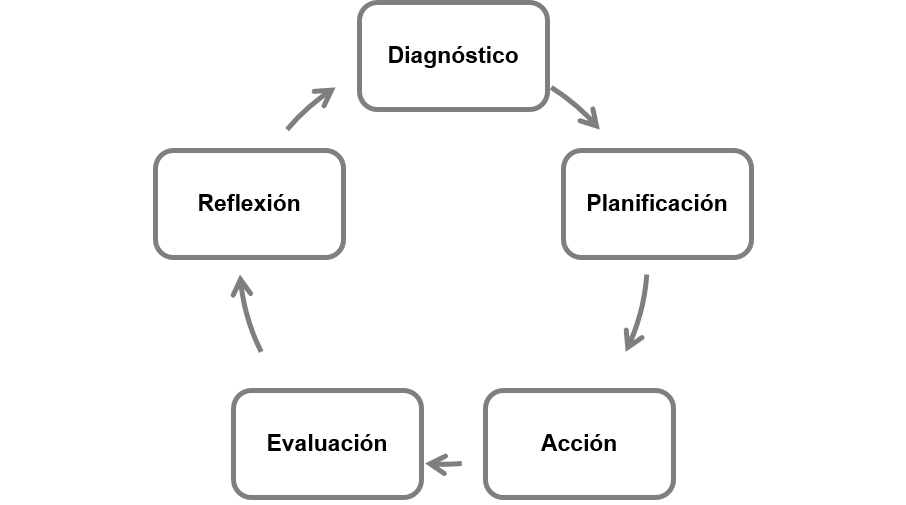
\includegraphics[scale=0.77]{img/investigacion-accion.png}
		\caption{\textbf{Figura 1.} \textit{Car\'{a}cter c\'{i}clico de Investigaci\'{o}n-Acci\'{o}n} (Fuente: Baskerville, 1999).}
\end{figure}
\FloatBarrier %you shall not pass table!!
\begin{itemize}
	\item \textbf{Fase de diagn\'{o}stico:} Se realiza el proceso de identificaci\'{o}n de los problemas primarios de la investigaci\'{o}n.
	\item \textbf{Fase de planificaci\'{o}n:} Se especifican las acciones que se llevaran a cabo para solucionar los problemas primarios.
	\item \textbf{Fase de acci\'{o}n:} Se ejecutan las acciones planificadas en la fase anterior.
	\item \textbf{Fase de evaluaci\'{o}n u observaci\'{o}n:} Se efect\'{u}a una evaluaci\'{o}n de los resultados obtenidos, para observar, conocer y documentar los efectos de las acciones que fueron realizadas.
	\item \textbf{Fase de reflexi\'{o}n:} Se toman los conocimientos adquiridos en la investigaci\'{o}n-acci\'{o}n. Si las acciones ejecutadas no fueron exitosas, los conocimientos pueden proporcionar la base para el diagn\'{o}stico de un nuevo ciclo de investigaci\'{o}n-acci\'{o}n.
\end{itemize}

En la Tabla 2 se muestran las actividades del presente proyecto, haciendo correspondencia a cada una de las fases de la Investigaci\'{o}n-Acci\'{o}n.
\FloatBarrier %you shall not pass table!!
\begin{table}[htb]
	\small
	\centering
	\setlength{\extrarowheight}{5pt}
	\begin{tabulary}{15cm}{|c|L|}
		\hline
		\textbf{Fase} & \textbf{Actividades}\\ \hline
		\textbf{Diagn\'{o}stico} & Identificar los problemas y limitaciones que presenta el software comercial del ``Miniscan XE PLUS''.\\ \hline
		\textbf{Planificaci\'{o}n} & Seleccionar la metodolog\'{i}a de desarrollo, determinar los requisitos del software y realizar un plan de trabajo.
\\ \hline
		\textbf{Acci\'{o}n} & Desarrollar el software, tomando en cuenta los requisitos identificados previamente, los lineamientos de ingenier\'{i}a del software, est\'{a}ndares de dise\~{n}o y calidad de software.\\ \hline
		\textbf{Evaluaci\'{o}n} & Realizar las pruebas de funcionalidad del software en cuesti\'{o}n y de su interfaz gr\'{a}fica de usuario.\\ \hline
		\textbf{Reflexi\'{o}n} & Presentar los resultados y los an\'{a}lisis de las pruebas realizadas.\\ \hline
	\end{tabulary}
	\caption{\textbf{Tabla 2.} \textit{Actividades del proyecto seg\'{u}n metodolog\'{i}a Investigaci\'{o}n-Acci\'{o}n }		(Fuente: Elaboración propia).}
\end{table}
\FloatBarrier %you shall not pass table!!
	\subsection{Metodolog\'{i}a de desarrollo de software}
Para el desarrollo del software que cumpla con los objetivos planteados en esta investigaci\'{o}n y tomando en cuenta los lineamientos planteados por la ingenier\'{i}a del software, con el objetivo de obtener un software que sea fiable y que funcione eficientemente (Pressman, 2002), se ha realizado una revisi\'{o}n del enfoque que deber\'{i}a tener la metodolog\'{i}a de desarrollo a utilizar.

Seg\'{u}n Sommerville (2005, p. 361), en los a\~{n}os 80 y principios de los 90, exist\'{i}a una opini\'{o}n general de que la mejor forma de obtener un mejor software era a trav\'{e}s de una planificaci\'{o}n cuidadosa del proyecto, una garant\'{i}a de calidad formalizada, la utilizaci\'{o}n de m\'{e}todos de an\'{a}lisis y dise\~{n}o soportados por herramientas CASE, y procesos de desarrollo de software controlados y rigurosos. El software que segu\'{i}a lo mencionado previamente era desarrollado por grandes equipos que a veces trabajaban para compa\~{n}\'{i}as diferentes. A menudo estaban dispersos geogr\'{a}ficamente y trabajaban en el software durante largos periodos de tiempo.

Ahora bien, debido a que no se dispone de un equipo grande para el desarrollo del software objetivo de la presente investigaci\'{o}n, y a que no se trabajar\'{a} en \'{e}ste durante un largo periodo de tiempo, se utilizar\'{a} una metodolog\'{i}a de desarrollo de enfoque \'{a}gil. Acorde con Sommerville (2005, p. 362), los m\'{e}todos \'{a}giles dependen de un enfoque iterativo para la especificaci\'{o}n, desarrollo y entrega del software, y est\'{a}n pensados para entregar software funcional de forma r\'{a}pida a los clientes, quienes pueden entonces proponer que se incluyan en iteraciones posteriores del software nuevos requerimientos o cambios en los mismos. Si bien los m\'{e}todos \'{a}giles proponen procesos diferentes para el desarrollo y entrega incrementales de software, comparten un conjunto de principios en com\'{u}n, los cuales son ilustrados en la Tabla 3.

\begin{table}[htb]
	\small
	\centering
	\setlength{\extrarowheight}{5pt}
	\begin{tabulary}{15cm}{|c|L|}
		\hline
		\textbf{Principio} & \textbf{Descripci\'{o}n}\\ \hline
		\textbf{Participaci\'{o}n del cliente} & Los clientes deben estar fuertemente implicados en todo el proceso de desarrollo. Su papel es proporcionar y priorizar nuevos requerimientos del software y evaluar las iteraciones del sistema.\\ \hline
		\textbf{Entrega incremental} & El software se desarrolla en incrementos, donde el cliente especifica los requerimientos a incluir en cada incremento.\\ \hline
		\textbf{Personas, no procesos} & Se deben reconocer y explotar las habilidades del equipo de desarrollo. Se les debe dejar desarrollar sus propias formas de trabajar, sin procesos formales.\\ \hline
		\textbf{Aceptar el cambio} & Se debe contar con que los requerimientos del software cambian, por lo que el software se dise\~{n}a para dar cabida a estos cambios.\\ \hline
		\textbf{Mantener la simplicidad} & Se debe centrar la simplicidad tanto en el software a desarrollar como en el proceso de desarrollo. Donde sea posible, se trabaja activamente para eliminar la complejidad del software.\\ \hline
	\end{tabulary}
	\caption{\textbf{Tabla 3.} \textit{Principios de los m\'{e}todos \'{a}giles} (Fuente: Sommerville, 2005).}
\end{table}

	\subsubsection{Metodolog\'{i}a SCRUM}
	
De acuerdo con Schwaber y Sutherland (2013, p. 4), esta metodolog\'{i}a es un marco de trabajo por el cual las personas pueden acometer problemas complejos adaptativos, y a la vez entregar productos del m\'{a}ximo valor posible, productiva y creativamente. SCRUM no es un proceso o una t\'{e}cnica para construir productos; en lugar de eso, es un marco de trabajo dentro del cual se pueden emplear varias t\'{e}cnicas y procesos. 
El marco de trabajo SCRUM consiste en los equipos SCRUM, roles, eventos, artefactos y reglas asociadas. Cada componente dentro del marco de trabajo sirve a un prop\'{o}sito espec\'{i}fico y es esencial para el \'{e}xito de SCRUM y para su uso (Schwaber y Sutherland, 2013, p. 4).

SCRUM se basa en la teor\'{i}a de control de procesos emp\'{i}rica. El empirismo asegura 	que el conocimiento procede de la experiencia y de tomar decisiones bas\'{a}ndose en lo que se conoce. Esta metodolog\'{i}a emplea un enfoque iterativo e incremental para optimizar la predictibilidad y el control de riesgo. La implementaci\'{o}n de este control de procesos est\'{a} soportada por tres pilares, los cuales se muestran en la Tabla 4.

\begin{table}[htb]
	\small
	\centering
	\setlength{\extrarowheight}{5pt}
	\begin{tabulary}{15cm}{|c|L|}
		\hline
		\textbf{Pilar} & \textbf{Descripci\'{o}n}\\ \hline
		\textbf{Transparencia} & Los aspectos significativos del proceso deben ser visibles para aquellos que son responsables del resultado.\\ \hline
		\textbf{Inspecci\'{o}n} & Los usuarios SCRUM deben inspeccionar frecuentemente los artefactos de SCRUM y el proceso hacia un objetivo, para detectar variaciones.\\ \hline
		\textbf{Adaptaci\'{o}n} & Si un inspector determina que uno o m\'{a}s aspectos de un proceso se desv\'{i}an de l\'{i}mites aceptables, y que el producto resultante no ser\'{a} aceptable, el proceso o el material que est\'{a} siendo procesado debe ser ajustado.\\ \hline
	\end{tabulary}
	\caption{\textbf{Tabla 4.} \textit{Pilares del control de procesos de SCRUM} (Fuente: Elaboraci\'{o}n propia).}
\end{table}

Adicionalmente a la utilizaci\'{o}n de la metodolog\'{i}a SCRUM, se incluyeron algunos
artefactos de la metodolog\'{i}a RUP (Rational Unified Process), para as\'{i} generar suficiente documentaci\'{o}n durante el dise\~{n}o y el desarrollo del nuevo software. La configuraci\'{o}n
 de la metodolog\'{i}a SCRUM utlizada en conjunto con los artefactos elegidos de la
 metodolog\'{i}a RUP, es la ilustrada en la Tabla 5.

\begin{table}[htb]
	\small
	\centering
	\setlength{\extrarowheight}{5pt}
	\begin{tabulary}{15cm}{|L|L|}
		\hline
		\textbf{Artefactos SCRUM}\\ \hline
		\textbf{Backlog de producto:} Lista din\'{a}mica de las cosas que se deben hacer, sin especificar c\'{o}mo se deben hacer.\\ \hline
		\textbf{Backlog de sprint:} Recopilaci\'{o}n sint\'{e}tica de los \'{i}tems del backlog del producto, en donde se quiebran los \'{i}tems en tareas peque\~{n}as que no demanden una labor superior a una jornada de trabajo.\\ \hline
		\textbf{Incremento de funcionalidad:} Es lo que el equipo SCRUM entrega la final de cada sprint. El mismo debe asemejarse a un software funcionando, permitiendo implementarse operativamente sin restricciones en un ambiente productivo.\\ \hline
		\textbf{Artefactos RUP}\\ \hline
		\textbf{Documento de Visi\'{o}n:}...\\ \hline
		\textbf{Glosario:}...\\ \hline
		\textbf{Configuraci\'{o}n de documentos de requerimientos:} Solamente requerimientos no funcionales.\\ \hline
		\textbf{Configuraci\'{o}n de documentos de arquitectura:} Solamente diagrama de Casos de Uso.\\ \hline
	\end{tabulary}
	\caption{\textbf{Tabla 5.} \textit{Configuraci\'{o}n de los artefactos a utilizar de SCRUM y RUP} (Fuente: Elaboraci\'{o}n propia).}
\end{table}

\end{document}